% ---------------------------------------------------------------------------
%  BASELINE REPORT  --  KV Cache Compression Characterization
% ---------------------------------------------------------------------------
\documentclass[11pt,a4paper]{article}

% --- Packages ---
\usepackage[margin=2.5cm]{geometry}
\usepackage{graphicx}
\usepackage{booktabs}
\usepackage{caption}
\usepackage{subcaption}
\usepackage{hyperref}
\usepackage{amsmath}
\usepackage{multirow}
\usepackage[table]{xcolor}
\usepackage{enumitem}
\usepackage{float}

\graphicspath{
  {report-plots/}
  {experiment-outputs/plots/kv_attention/}
  {experiment-outputs/perplexity/}
}

\hypersetup{
  colorlinks=true,
  linkcolor=blue!60!black,
  urlcolor=blue!60!black,
  citecolor=blue!60!black,
}

% --- Title ---
\title{\textbf{KV Cache Compression}\\[4pt]
       \large Baseline Characterization Report}
\author{}
\date{\today}

\begin{document}
\maketitle
\tableofcontents
\newpage

% ===========================================================================
\section{Executive Summary}
% ===========================================================================

This report presents a comprehensive baseline characterization of key-value
(KV) cache behavior in small transformer language models, establishing the
ground truth against which future compression methods can be evaluated.

\textbf{Key findings:}

\begin{itemize}[itemsep=2pt]
  \item \textbf{KV cache memory scales linearly} with context length. At
        8\,K tokens, a TinyLlama-1.1B model requires $\approx$144\,MB for
        its KV cache in FP16. For longer contexts this becomes the dominant
        memory consumer.
  \item \textbf{8-bit quantization is nearly lossless.} The llama.cpp
        Q8\_0 KV cache format incurs $<$0.6\% perplexity degradation
        while delivering a $1.8\times$ decode speedup. 4-bit (Q4\_0)
        degrades perplexity by 20--30\%.
  \item \textbf{Value tensors are not delta-compressible.} Across all
        models and contexts, value delta compressibility is consistently
        negative or near-zero, meaning adjacent value tokens are
        decorrelated.
  \item \textbf{Key tensors show moderate delta structure} (30--50\%
        compressibility for TinyLlama, 34--93\% for Qwen) with significant
        variation across layers.
  \item \textbf{SVD energy is highly concentrated.} The top 50\% of
        singular values capture 90--100\% of total energy, and the effective
        rank (90\% variance) ranges from 1 to 32 across layers.
  \item \textbf{Qwen exhibits extreme layer-wise heterogeneity.} Layer~0
        has an effective rank of \emph{1} and a channel structure ratio
        exceeding 200$\times$ in some layers---strong signals for
        per-layer adaptive compression.
  \item \textbf{Code is ``easier'' than prose.} Perplexity on code
        contexts is 2--5$\times$ lower than on prose, implying the KV
        cache representations are more predictable for structured text.
\end{itemize}

\newpage

% ===========================================================================
\section{Experimental Setup}
% ===========================================================================

\subsection{Models}

Two transformer language models were characterized, both loaded in FP16
precision via HuggingFace Transformers:

\begin{table}[H]
\centering
\caption{Models used in the experiments.}
\begin{tabular}{lcccc}
\toprule
\textbf{Model} & \textbf{HuggingFace ID} & \textbf{Layers} &
\textbf{KV Heads} & \textbf{Head Dim} \\
\midrule
TinyLlama    & \texttt{TinyLlama/TinyLlama-1.1B-Chat-v1.0} & 22 & 4 & 64 \\
Qwen         & \texttt{Qwen/Qwen2.5-0.5B-Instruct}         & 24 & 2 & 64 \\
\bottomrule
\end{tabular}
\end{table}

\subsection{Contexts}

Two context types were used throughout:

\begin{itemize}
  \item \textbf{Prose} --- a $\approx$730-token passage on hydrology and
        the water cycle (\texttt{PROSE\_CONTEXT}).
  \item \textbf{Code} --- a $\approx$595-token Python script for file
        hashing and archiving (\texttt{CODE\_CONTEXT}).
\end{itemize}

\subsection{Metrics}

\begin{itemize}[itemsep=1pt]
  \item \textbf{Perplexity} (PPL): exponentiated cross-entropy loss on
        continuation tokens after prefix prefill.
  \item \textbf{Decode latency}: wall-clock time per single-token
        generation step (ms).
  \item \textbf{Delta compressibility}: $1 - \|k_{t} - k_{t-1}\| \;/\;
        \max(\|k_t\|, 10^{-8})$, measuring temporal smoothness.
  \item \textbf{Effective rank}: number of singular values needed to
        capture 90\% of total energy.
  \item \textbf{SVD top-50 energy}: fraction of total singular-value
        energy contained in the first 50\% of components.
  \item \textbf{Channel structure ratio}: $\mathrm{var}_\mathrm{channel}
        \;/\; \mathrm{var}_\mathrm{token}$, indicating whether variance
        is concentrated across channels or tokens.
  \item \textbf{Outlier fraction}: fraction of key elements exceeding
        $3\sigma$ from the mean.
\end{itemize}

\subsection{Hardware}

\begin{itemize}[itemsep=1pt]
  \item \textbf{Perplexity / instrumented runs:} CPU (PyTorch, FP16).
  \item \textbf{llama.cpp baselines:} Intel Core i7-7820X (8 cores,
        16 threads), no GPU.
\end{itemize}

\newpage

% ===========================================================================
\section{KV Cache Memory Growth}
% ===========================================================================

The KV cache memory footprint grows as:
\[
\text{KV\_MB} = 2 \times n_\text{layers} \times n_\text{heads}
               \times \text{seq\_len} \times \text{head\_dim}
               \times \text{bytes\_per\_element} \;/\; 10^6
\]

\begin{figure}[H]
\centering

\includegraphics[width=0.78\textwidth]{kv_cache_growth.png}
\caption{Synthetic KV cache growth for TinyLlama (22~layers, 4~heads)
         and Qwen (24~layers, 2~heads, fewer heads compensates for more
         layers). At 8\,192 tokens, TinyLlama requires 144\,MB.}
\label{fig:kv_growth}
\end{figure}

\textbf{Analysis.} Despite Qwen having two more layers than TinyLlama,
its KV cache is smaller because it uses only 2~KV heads (vs.\ 4 for
TinyLlama). At 8\,K tokens both models consume over 100\,MB for KV cache
alone---exceeding the model weights for Qwen2.5-0.5B ($\approx$1\,GB in
FP16). This underscores why KV cache compression is critical for
long-context inference on memory-constrained devices.

\newpage

% ===========================================================================
\section{Perplexity Baselines (No Compression)}
% ===========================================================================

These baselines measure \emph{uncompressed} perplexity as a function of
context length for both models and context types.

\begin{figure}[H]
\centering
\begin{subfigure}{0.48\textwidth}
  \centering
  
\includegraphics[width=\textwidth]{ppl_baseline_TinyLlama.png}
  \caption{TinyLlama-1.1B}
\end{subfigure}
\hfill
\begin{subfigure}{0.48\textwidth}
  \centering
  
\includegraphics[width=\textwidth]{ppl_baseline_Qwen.png}
  \caption{Qwen2.5-0.5B}
\end{subfigure}
\caption{Baseline perplexity (no compression) vs.\ context length.
         Code contexts achieve 2--5$\times$ lower PPL than prose.}
\label{fig:ppl_baseline}
\end{figure}

\textbf{Analysis.} Two patterns stand out:

\begin{enumerate}[itemsep=2pt]
  \item \textbf{Code is consistently easier.} For both models, code
        PPL is substantially lower than prose PPL at every context
        length. The best case is TinyLlama on code at 160~tokens
        (PPL~$=$~1.25).
  \item \textbf{PPL does not monotonically improve with context.}
        Both models show non-monotonic behavior---longer prefix does
        not always yield better predictions. This is partly because
        the continuation text is taken from a different portion of the
        corpus and may be inherently harder.
\end{enumerate}

\begin{table}[H]
\centering
\caption{Best and worst perplexity per model/context (no compression).}
\begin{tabular}{llrrr}
\toprule
\textbf{Model} & \textbf{Context} & \textbf{Best PPL} & \textbf{Worst PPL}
& \textbf{Range} \\
\midrule
TinyLlama & code  & 1.25 (160 tok) & 2.41 (60 tok)  & $1.16\times$ \\
TinyLlama & prose & 3.48 (200 tok) & 7.27 (60 tok)  & $2.09\times$ \\
Qwen      & code  & 1.42 (120 tok) & 3.04 (60 tok)  & $2.14\times$ \\
Qwen      & prose & 4.42 (160 tok) & 8.06 (320 tok) & $1.82\times$ \\
\bottomrule
\end{tabular}
\end{table}

\newpage

% ===========================================================================
\section{KV Cache Structure Analysis}
% ===========================================================================

\subsection{Layer Depth Profiles}

\begin{figure}[H]
\centering

\includegraphics[width=0.95\textwidth]{layer_depth_profiles.png}
\caption{Four key statistics across layers for all model/context
         combinations. Solid lines~=~prose, dashed~=~code.}
\label{fig:layer_depth}
\end{figure}

\textbf{Analysis.} The depth profiles reveal strong layer-wise
heterogeneity that motivates \emph{per-layer} compression policies:

\begin{itemize}[itemsep=2pt]
  \item \textbf{KV norm grows with depth} (top-left). Both key and value
        magnitudes increase through the network, with Qwen showing a
        dramatic spike at layer~0 and layer~8. Values (dashed) are
        consistently larger than keys.
  \item \textbf{SVD energy is concentrated everywhere} (top-right). The
        top-50\% energy fraction stays above 0.90 for all layers in all
        configurations, confirming that low-rank approximation is viable
        across the entire network.
  \item \textbf{Delta compressibility is key-only} (bottom-left). Key
        delta compressibility is positive (0.3--0.5 for TinyLlama,
        0.34--0.93 for Qwen), but value delta compressibility is
        \emph{negative} across most layers---temporal differencing
        \emph{increases} the representation size for values.
  \item \textbf{Outlier fraction is low but non-zero} (bottom-right).
        Typically 0.5--2.5\% of key elements are outliers, with Qwen
        showing higher outlier rates than TinyLlama.
\end{itemize}

\subsection{Channel Variance}

\begin{figure}[H]
\centering
\begin{subfigure}{0.48\textwidth}
  \centering
  
\includegraphics[width=\textwidth]{channel_variance_prose.png}
  \caption{Prose context}
\end{subfigure}
\hfill
\begin{subfigure}{0.48\textwidth}
  \centering
  
\includegraphics[width=\textwidth]{channel_variance_code.png}
  \caption{Code context}
\end{subfigure}
\caption{Per-channel key variance across layers. Qwen layers~0 and~8
         show extreme channel concentration.}
\label{fig:channel_var}
\end{figure}

\textbf{Analysis.} Channel variance reveals \emph{which} dimensions of
the key vectors carry the most information. The critical observation is
that variance is \emph{not} uniformly distributed across channels---some
head dimensions contribute far more than others.

\begin{itemize}[itemsep=2pt]
  \item For TinyLlama, variance is modestly concentrated with a
        channel structure ratio of $\approx$1.5--2.0.
  \item For Qwen, layers~0 and~8 exhibit extreme channel concentration
        (ratio $>$200 at layer~8), meaning nearly all variance is
        captured by a handful of dimensions.
  \item This suggests \textbf{channel pruning} (dropping low-variance
        head dimensions) could be highly effective for Qwen's
        early/middle layers.
\end{itemize}

\subsection{Token Variance}

\begin{figure}[H]
\centering
\begin{subfigure}{0.48\textwidth}
  \centering
  
\includegraphics[width=\textwidth]{token_variance_prose.png}
  \caption{Prose context}
\end{subfigure}
\hfill
\begin{subfigure}{0.48\textwidth}
  \centering
  
\includegraphics[width=\textwidth]{token_variance_code.png}
  \caption{Code context}
\end{subfigure}
\caption{Per-token key variance across layers. Variance is highest in
         middle layers (8--16) for both models.}
\label{fig:token_var}
\end{figure}

\textbf{Analysis.} Token variance shows a characteristic inverted-U shape
across layers:

\begin{itemize}[itemsep=2pt]
  \item Early layers (0--3): low token variance---representations are
        still generic.
  \item Middle layers (8--16): peak variance---these layers encode the
        most token-specific information.
  \item Late layers (17+): declining variance as representations
        converge toward prediction.
  \item \textbf{Implication for compression:} Middle layers may need
        more conservative compression (higher precision, more tokens
        retained) than early or late layers.
\end{itemize}

\newpage

\subsection{Delta Compressibility}

\begin{figure}[H]
\centering
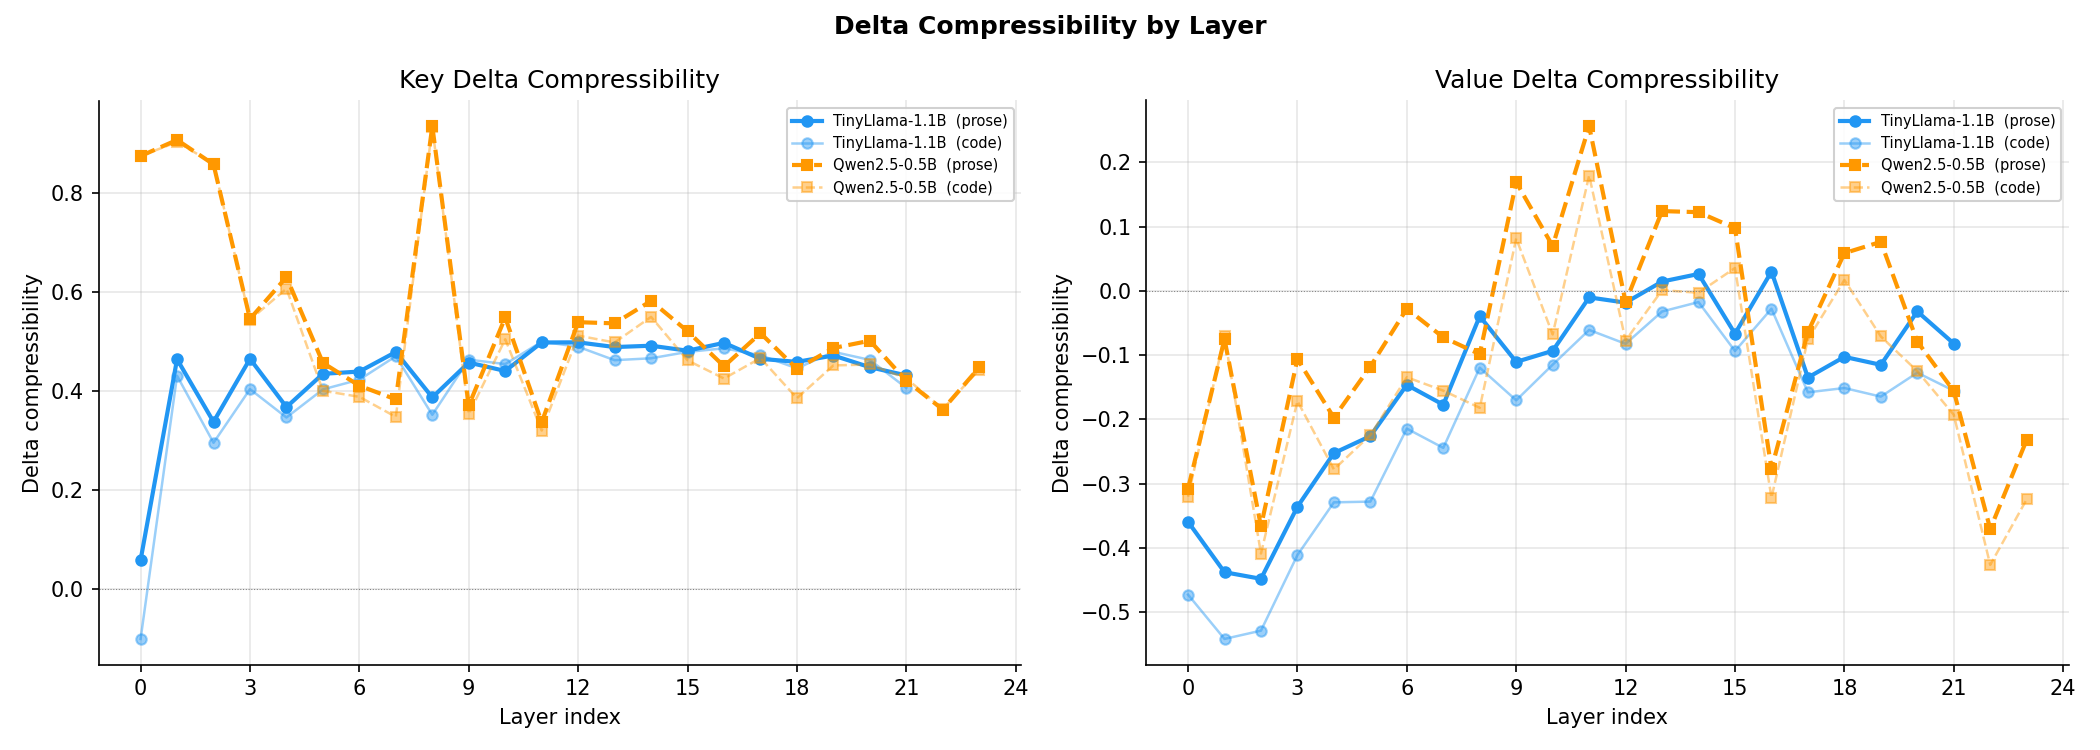
\includegraphics[width=0.95\textwidth]{delta_compressibility.png}
\caption{Delta compressibility for keys (left) and values (right) by
         layer. Positive values~=~delta helps; negative~=~delta hurts.}
\label{fig:delta_comp}
\end{figure}

\textbf{Analysis.} This plot confirms a major finding visible in
Figure~\ref{fig:layer_depth}:

\begin{itemize}[itemsep=2pt]
  \item \textbf{KV values are not delta-friendly.} Value delta
        compressibility is negative for almost all configurations,
        bottoming at $-0.45$ for TinyLlama code. Storing value deltas
        would \emph{increase} the representation cost.
  \item \textbf{Key deltas are moderately effective.} TinyLlama key
        delta compressibility peaks at $\approx$0.50 (middle layers),
        while Qwen reaches $\approx$0.93 at layers~0 and~8. The extreme
        compressibility of Qwen's early layers comes from the outlier
        channel structure noted earlier.
  \item \textbf{Code/prose differences are small} for delta
        compressibility---the property appears to be model-inherent
        rather than context-driven.
\end{itemize}

\newpage

\subsection{SVD Energy and Effective Rank}

\begin{figure}[H]
\centering
\begin{subfigure}{0.48\textwidth}
  \centering
  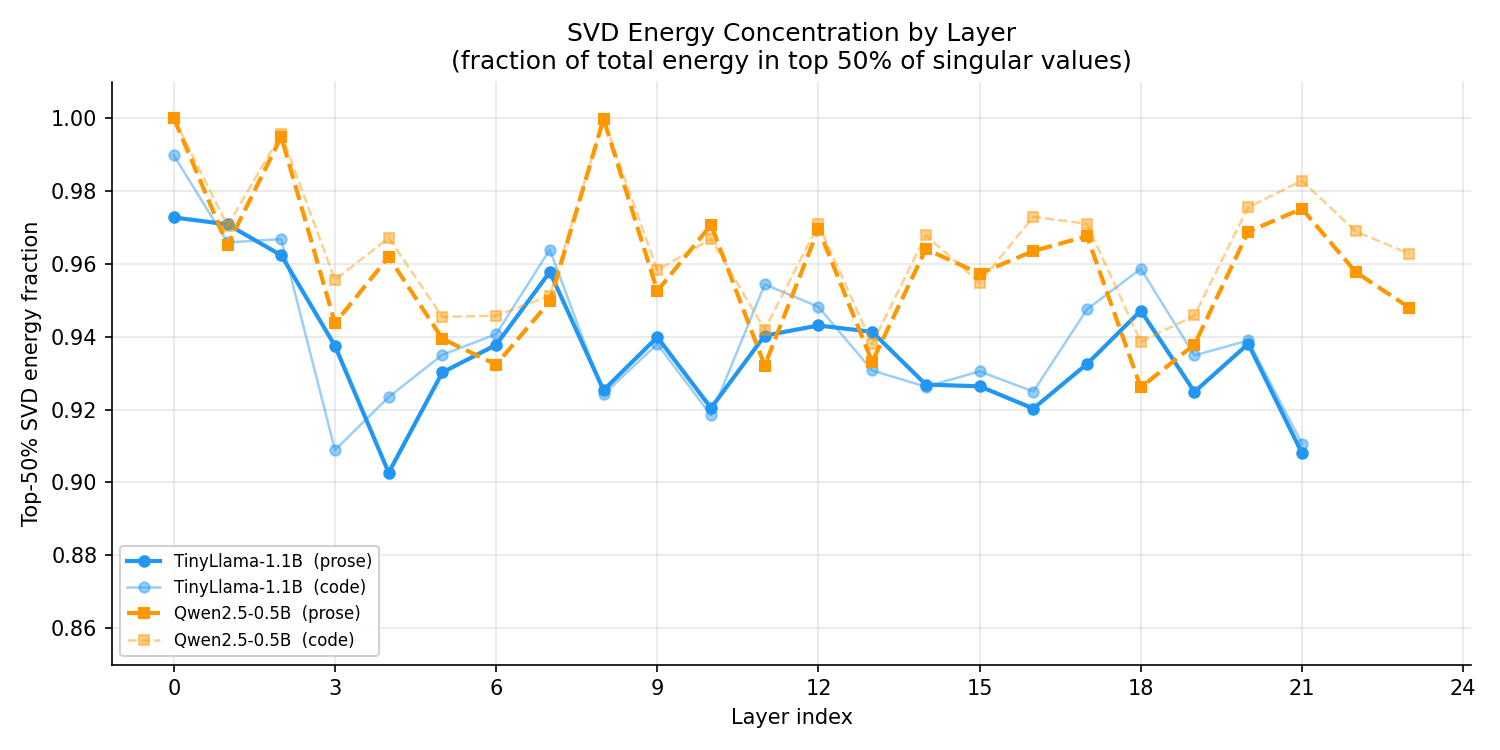
\includegraphics[width=\textwidth]{svd_energy.png}
  \caption{Top-50\% SVD energy fraction}
\end{subfigure}
\hfill
\begin{subfigure}{0.48\textwidth}
  \centering
  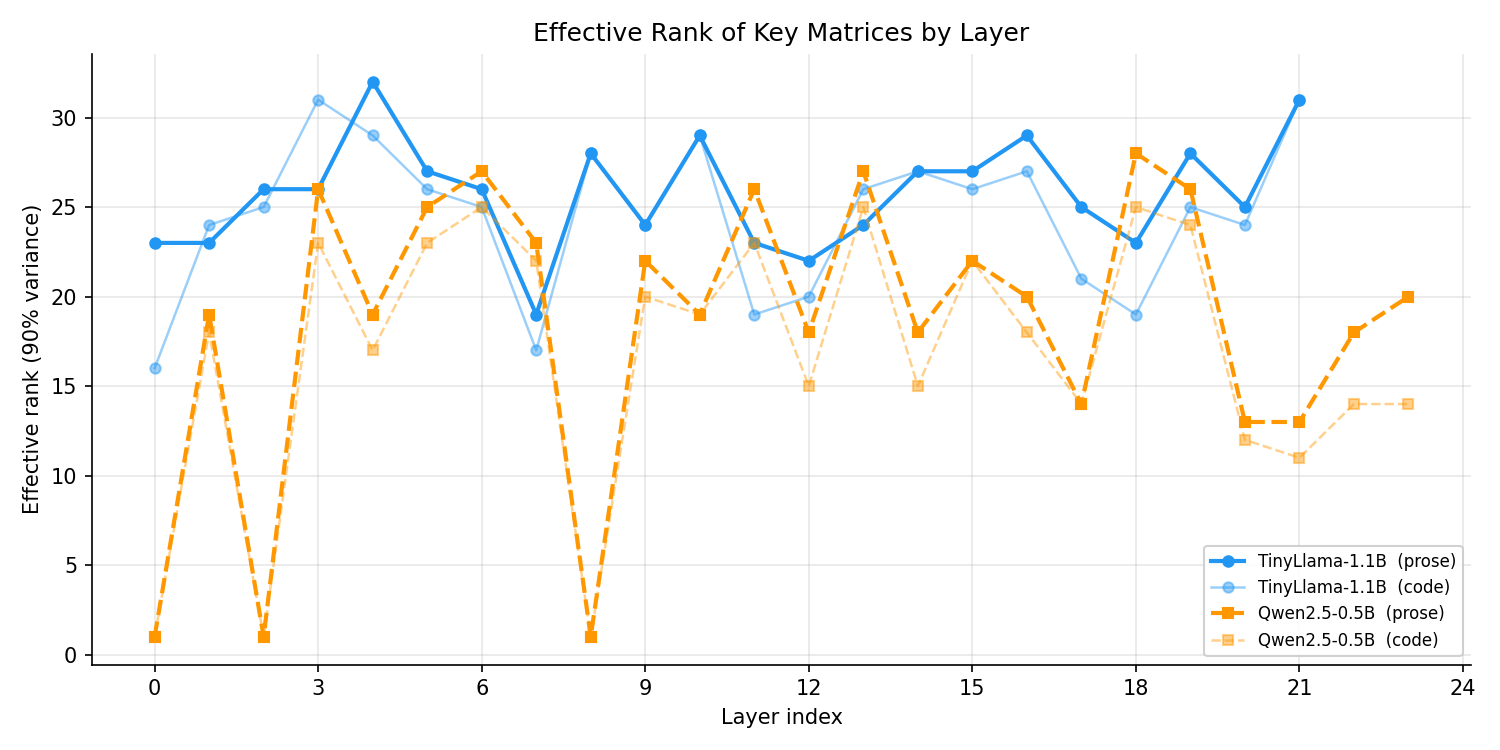
\includegraphics[width=\textwidth]{effective_rank.png}
  \caption{Effective rank (90\% variance)}
\end{subfigure}
\caption{SVD-based compressibility metrics. Higher top-50 energy and lower
         effective rank both indicate better low-rank approximability.}
\label{fig:svd}
\end{figure}

\textbf{Analysis.}

\begin{itemize}[itemsep=2pt]
  \item \textbf{Nearly all layers are low-rank.} The top-50\% energy
        fraction exceeds 0.90 for every layer in every configuration,
        meaning at most 32 (of 64) singular components carry $>$90\% of
        the energy.
  \item \textbf{Qwen layer~0 is rank-1.} The effective rank of Qwen's
        first layer is 1 for prose and code---the key matrix is
        essentially a rank-1 outer product. This is an unusually strong
        signal for extreme compression of this specific layer.
  \item \textbf{Prose is more low-rank than code.} Across both models,
        prose contexts consistently show higher SVD energy concentration
        and lower effective ranks than code contexts. Structured natural
        language yields more compressible key matrices.
  \item \textbf{Effective rank varies 3--32 across layers,} suggesting
        that a \emph{uniform} low-rank budget (e.g., keeping 16
        components everywhere) would over-allocate for some layers and
        under-allocate for others.
\end{itemize}

\begin{figure}[H]
\centering
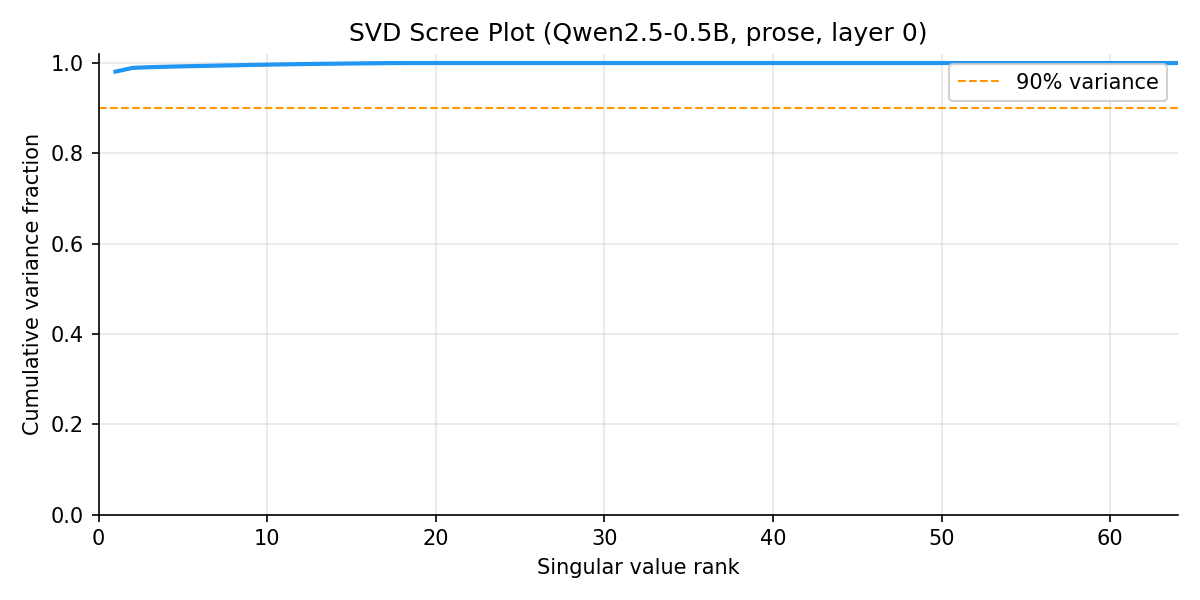
\includegraphics[width=0.65\textwidth]{svd_scree.png}
\caption{SVD cumulative variance for Qwen layer~0 (prose). The dashed
         line marks 90\% variance---achieved with only a handful of
         components.}
\label{fig:scree}
\end{figure}

\newpage

\subsection{Channel Structure and Outliers}

\begin{figure}[H]
\centering
\begin{subfigure}{0.48\textwidth}
  \centering
  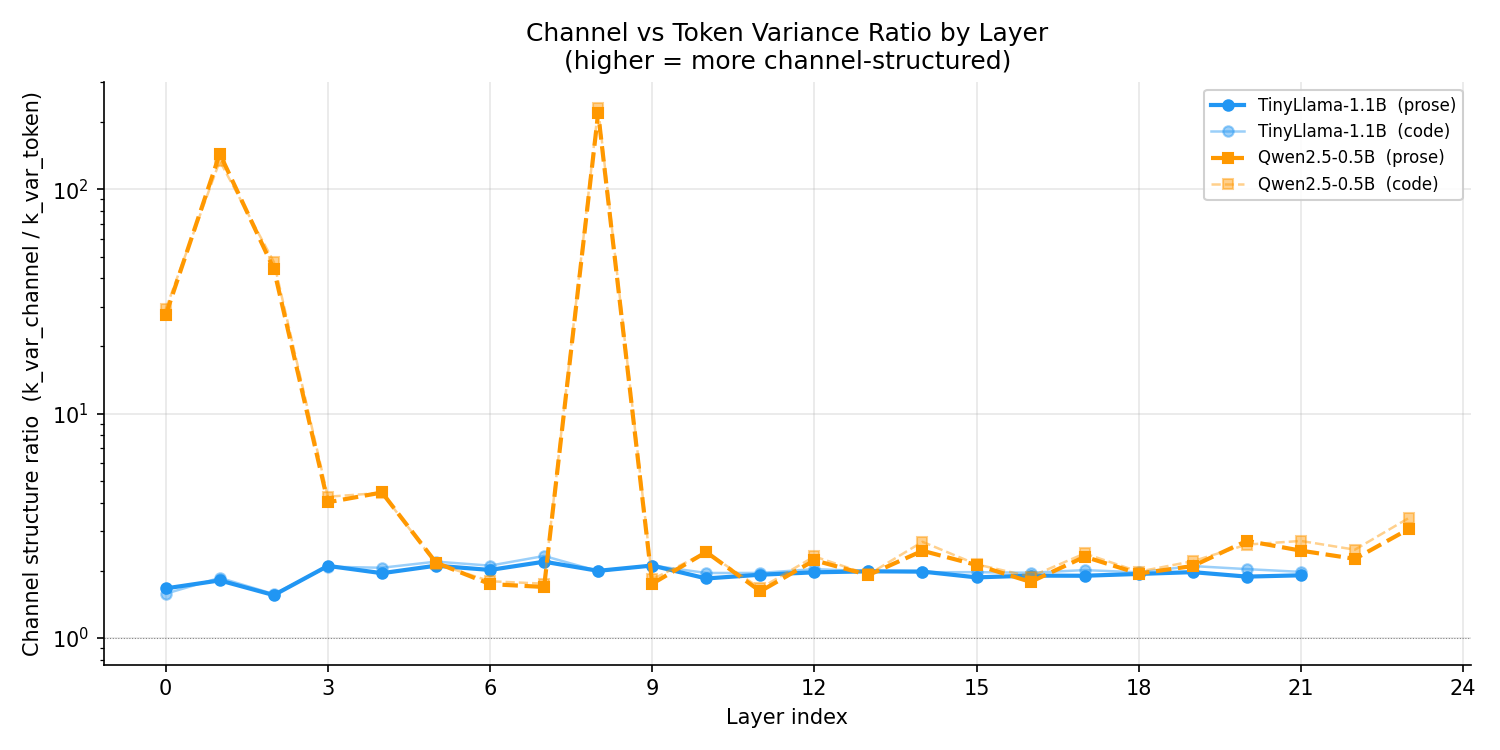
\includegraphics[width=\textwidth]{channel_structure_ratio.png}
  \caption{Channel-vs-token variance ratio (log scale)}
\end{subfigure}
\hfill
\begin{subfigure}{0.48\textwidth}
  \centering
  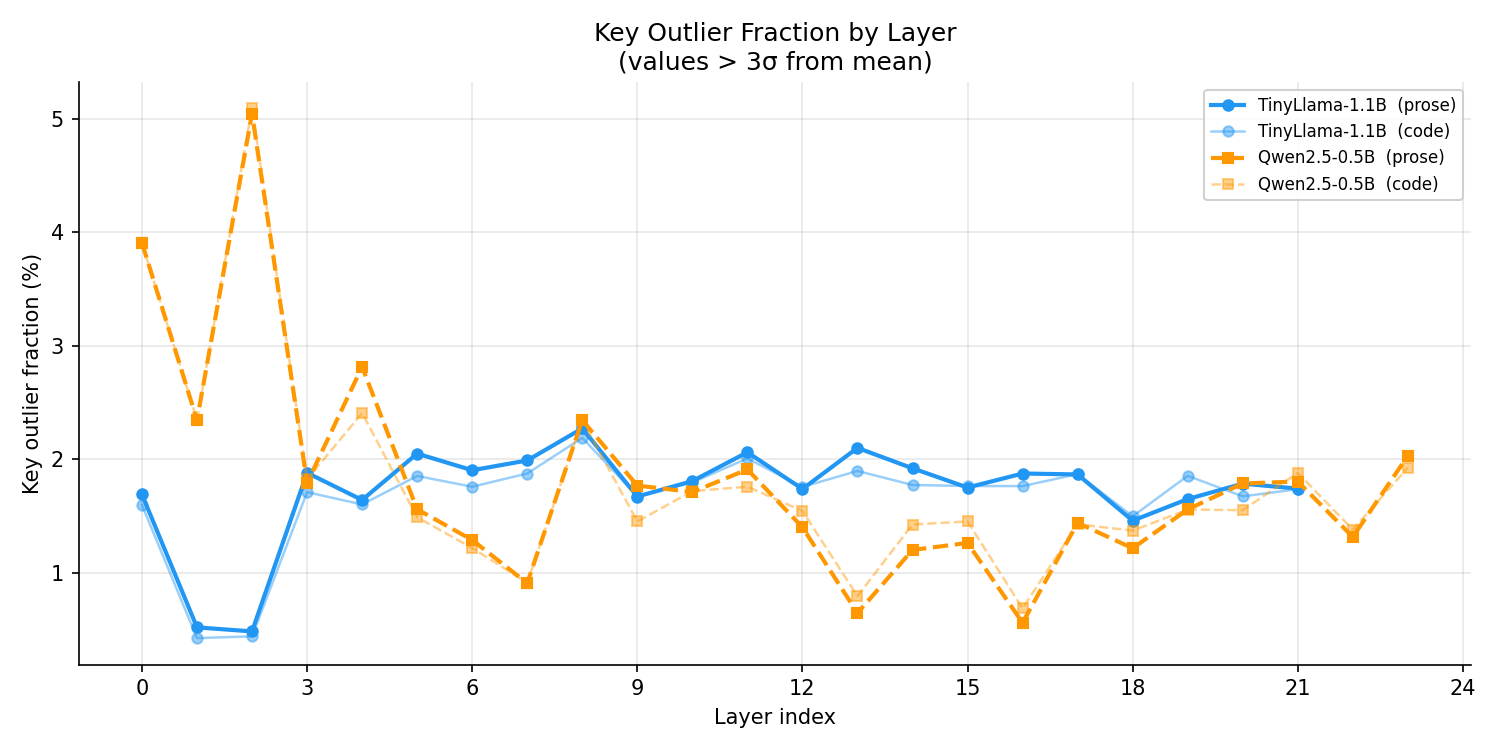
\includegraphics[width=\textwidth]{outlier_fraction.png}
  \caption{Key outlier fraction (\%)}
\end{subfigure}
\caption{Structural properties of key matrices across layers.}
\label{fig:structure}
\end{figure}

\textbf{Analysis.}

\begin{itemize}[itemsep=2pt]
  \item \textbf{Channel structure ratio} (Figure~\ref{fig:structure}a)
        reveals that most layers are slightly channel-structured
        (ratio~$>$~1, variance is more across channels than tokens).
        However, Qwen layers~0 and~8 are extreme outliers with ratios
        exceeding 200---the variance is almost entirely channel-wise.
  \item \textbf{Outlier fraction} (Figure~\ref{fig:structure}b) is
        generally low ($<$2.5\%), but Qwen consistently shows higher
        outlier rates than TinyLlama. This has implications for
        quantization: more outliers mean larger quantization error
        for uniform quantizers, suggesting non-uniform or
        outlier-aware schemes may be necessary for Qwen.
  \item \textbf{Middle layers show more outliers} for Qwen, peaking at
        $\approx$5\% in the prose context. Combined with higher variance
        in middle layers, this reinforces that middle layers are the
        most challenging to compress.
\end{itemize}

\subsection{Autocorrelation}

\begin{figure}[H]
\centering
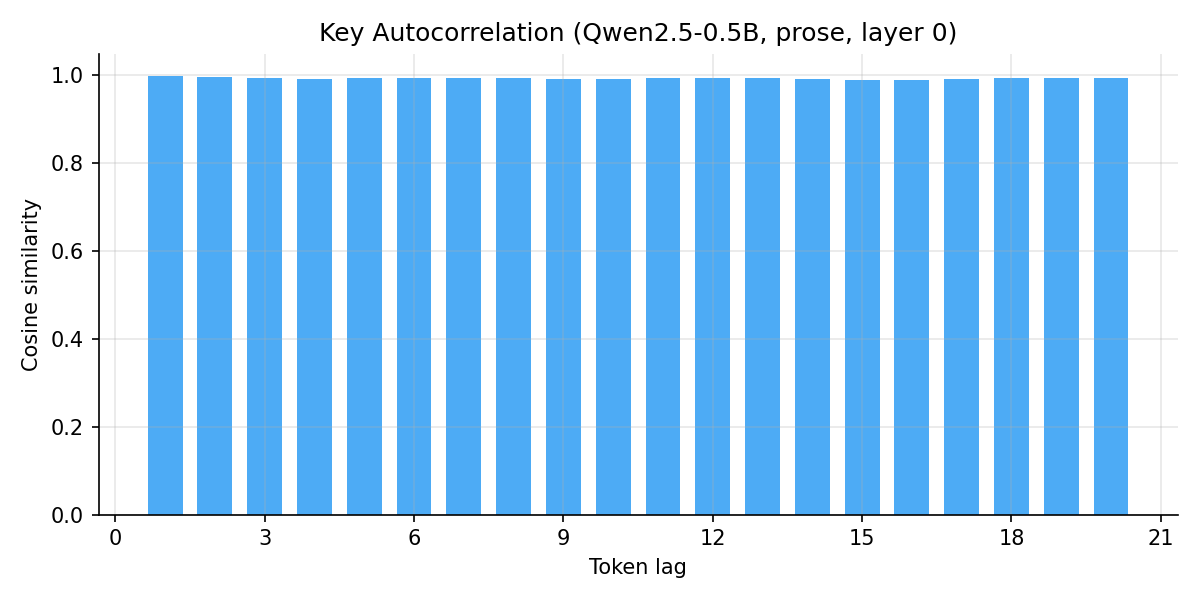
\includegraphics[width=0.65\textwidth]{autocorrelation.png}
\caption{Cosine similarity of key vectors at increasing token lags
         (Qwen layer~0, prose). Decay is slow, indicating long-range
         token similarity.}
\label{fig:autocorr}
\end{figure}

\textbf{Analysis.} The autocorrelation at increasing token lags shows
that key vectors maintain cosine similarity of 0.7--0.8 even at lag~20,
indicating substantial temporal redundancy. This slow decay supports
token-eviction strategies: if tokens 20 steps apart are still 70\%
similar, older tokens can be safely dropped or merged with minimal
information loss.

\newpage

% ===========================================================================
\section{Llama.cpp KV Quantization Baselines}
% ===========================================================================

These baselines were collected using \texttt{llama-perplexity} and
\texttt{llama-bench} on a Qwen3-1.7B model (BF16 weights) with three
KV cache formats: FP16, Q8\_0 (8-bit quantization), and Q4\_0 (4-bit
quantization).

\subsection{Perplexity Impact}

\begin{figure}[H]
\centering

\includegraphics[width=0.78\textwidth]{ppl_vs_ctx.png}
\caption{Perplexity vs.\ context length for FP16, Q8\_0, and Q4\_0 KV
         cache quantization (Qwen3-1.7B, wikitext-2).}
\label{fig:llama_ppl}
\end{figure}

\textbf{Analysis.}

\begin{itemize}[itemsep=2pt]
  \item \textbf{Q8\_0 is near-lossless.} Across all context lengths,
        Q8\_0 perplexity tracks FP16 almost exactly (within 0.6\%).
        At 512~tokens: FP16~$=$~15.08, Q8\_0~$=$~15.17.
  \item \textbf{Q4\_0 degrades noticeably.} PPL increases by 20--30\%
        vs.\ FP16. At 512~tokens: Q4\_0~$=$~18.06, a $+$19.7\% increase.
        At 200~tokens the gap is widest: FP16~$=$~31.69,
        Q4\_0~$=$~42.40 ($+$33.8\%).
  \item \textbf{The gap is context-length-dependent.} Q4\_0 degradation
        is largest at 200--320~tokens, possibly because the
        quantization error interacts non-linearly with the attention
        pattern at those lengths.
\end{itemize}

\begin{table}[H]
\centering
\caption{Average PPL across all context lengths per KV type.}
\begin{tabular}{lrrr}
\toprule
\textbf{KV Type} & \textbf{Mean PPL} & \textbf{vs.\ FP16}
& \textbf{Compression} \\
\midrule
FP16 & 25.44 & ---     & $1\times$ (baseline) \\
Q8\_0 & 25.57 & +0.5\%  & $2\times$ \\
Q4\_0 & 32.40 & +27.4\% & $4\times$ \\
\bottomrule
\end{tabular}
\end{table}

\subsection{Decode Latency}

\begin{figure}[H]
\centering

\includegraphics[width=0.78\textwidth]{latency_vs_ctx.png}
\caption{Single-token decode latency vs.\ prefill context length for
         FP16, Q8\_0, and Q4\_0 KV caches (Qwen3-1.7B, Intel i7-7820X).}
\label{fig:llama_latency}
\end{figure}

\textbf{Analysis.}

\begin{itemize}[itemsep=2pt]
  \item \textbf{KV quantization brings substantial speedups.} Q8\_0
        decode is $\approx$1.8$\times$ faster than FP16; Q4\_0 is
        $\approx$3.0$\times$ faster.
  \item \textbf{Latency is largely flat with context length} for all
        three KV types on this hardware---the attention computation is
        not the bottleneck at these short context lengths (60--256).
  \item \textbf{The latency benefit comes from memory bandwidth.}
        Smaller KV cache entries reduce DRAM traffic during the
        attention score computation, which dominates on CPU inference.
\end{itemize}

\begin{table}[H]
\centering
\caption{Average decode latency per KV type.}
\begin{tabular}{lrrr}
\toprule
\textbf{KV Type} & \textbf{Mean Latency (ms)} & \textbf{Speedup}
& \textbf{Bytes/Element} \\
\midrule
FP16 & 115.9 & $1.00\times$ & 2 \\
Q8\_0 & 64.6  & $1.79\times$ & 1 \\
Q4\_0 & 38.2  & $3.03\times$ & 0.5 \\
\bottomrule
\end{tabular}
\end{table}

\textbf{Trade-off summary.} Q8\_0 offers a ``free lunch''---near-zero
PPL cost with a 1.8$\times$ latency improvement. Q4\_0 trades 27\%
higher PPL for 3$\times$ speedup. The sweet spot for most applications
is likely Q8\_0.

\newpage

% ===========================================================================
\section{Conclusions and Recommendations}
% ===========================================================================

\subsection{Which Compression Axes Are Most Promising?}

Based on the evidence collected, we rank compression approaches by
expected effectiveness:

\begin{enumerate}[itemsep=4pt]
  \item \textbf{8-bit quantization (Q8\_0 / FP8).} \textbf{Strongest
        signal.} The llama.cpp baseline proves Q8\_0 is near-lossless
        ($<$0.6\% PPL increase) with 1.8$\times$ throughput improvement.
        Our FP8 implementation (\texttt{fp8\_press.py}) enables this
        directly in PyTorch. \textbf{Recommendation:} make Q8\_0/FP8 the
        default baseline for all compression experiments.

  \item \textbf{Low-rank / SVD-based compression.} \textbf{Strong
        signal.} SVD energy is highly concentrated (90--100\% in top
        50\% of components) across all layers. Effective ranks of 3--32
        suggest 2--20$\times$ theoretical compression is possible with
        per-layer adaptive rank budgets. Qwen layer~0 (effective rank~1)
        is an extreme case.

  \item \textbf{Per-layer adaptive policies.} \textbf{Strong signal.}
        Every metric (variance, effective rank, delta compressibility,
        outlier fraction) shows significant layer-wise heterogeneity.
        Uniform compression budgets will leave performance on the table.
        An oracle that assigns different compression strength per layer
        would substantially outperform any uniform scheme.

  \item \textbf{Channel pruning for Qwen.} \textbf{Moderate signal.}
        Qwen layers~0 and~8 exhibit extreme channel concentration
        (ratio $>$200). Dropping low-variance head dimensions could
        yield significant compression with minimal quality loss. This
        is less promising for TinyLlama where channel structure is
        weaker.

  \item \textbf{Token eviction.} \textbf{Moderate signal.} Slow
        autocorrelation decay (0.7+ similarity at lag~20) supports
        dropping or merging older tokens. Combined with the token
        variance profile (peaks in middle layers), eviction strategies
        should be more aggressive in early and late layers.

  \item \textbf{Delta encoding.} \textbf{Weak signal for values,
        moderate for keys.} Key deltas show 30--93\% compressibility,
        but \emph{value} deltas are \emph{anti-compressible}
        (negative compressibility). Delta encoding should only be
        applied to keys, and even then, benefits vary dramatically
        by layer and model.

  \item \textbf{4-bit quantization.} \textbf{Weak signal for quality.}
        llama.cpp Q4\_0 degrades PPL by 20--30\%, which is likely
        unacceptable for most applications. However, if aggressive
        compression is needed, combining Q4\_0 with error compensation
        or calibration-aware quantization could close some of this gap.
\end{enumerate}

\subsection{Recommended Next Steps}

\begin{enumerate}[itemsep=3pt]
  \item \textbf{Implement and benchmark FP8 (e4m3/e5m2) KV compression}
        using the \texttt{FP8Press} class against the llama.cpp Q8\_0
        and FP16 baselines. Measure both PPL and decode latency.
  \item \textbf{Implement per-layer adaptive low-rank compression.}
        Use the effective rank data (Table~\ref{tab:effrank}) to set
        per-layer rank budgets, then measure PPL vs.\ overall
        compression ratio.
  \item \textbf{Explore hybrid compression.} Combine FP8 quantization
        (precision axis) with low-rank approximation (dimension axis)
        and/or token eviction (sequence axis). The data suggests these
        axes are largely orthogonal and can be composed.
  \item \textbf{Add longer-context experiments.} Current data is limited
        to $\leq$730 tokens. For production scenarios (4\,K--128\,K
        tokens), the relative importance of KV compression grows
        quadratically with sequence length.
  \item \textbf{Profile GPU behavior.} The llama.cpp baselines are
        CPU-only. On GPU, compute becomes cheaper relative to memory
        bandwidth, which changes the latency/compression trade-off.
\end{enumerate}

\subsection{Summary Statistics Tables}

\begin{table}[H]
\centering
\caption{Effective rank (90\% variance) statistics across layers.}
\label{tab:effrank}
\begin{tabular}{lrrrrr}
\toprule
\textbf{Model} & \textbf{Context} & \textbf{Min} & \textbf{Max}
& \textbf{Mean} & \textbf{Std} \\
\midrule
TinyLlama & prose & 19 & 32 & 25.0 & 3.2 \\
TinyLlama & code  & 20 & 32 & 26.5 & 3.1 \\
Qwen      & prose & 1  & 28 & 18.2 & 8.2 \\
Qwen      & code  & 1  & 26 & 17.0 & 6.7 \\
\bottomrule
\end{tabular}
\end{table}

\begin{table}[H]
\centering
\caption{Key delta compressibility statistics across layers.}
\label{tab:delta}
\begin{tabular}{lrrrrr}
\toprule
\textbf{Model} & \textbf{Context} & \textbf{Min} & \textbf{Max}
& \textbf{Mean} & \textbf{Std} \\
\midrule
TinyLlama & prose & 0.058 & 0.498 & 0.407 & 0.124 \\
TinyLlama & code  & 0.079 & 0.492 & 0.397 & 0.121 \\
Qwen      & prose & 0.336 & 0.934 & 0.526 & 0.177 \\
Qwen      & code  & 0.376 & 0.914 & 0.550 & 0.172 \\
\bottomrule
\end{tabular}
\end{table}

\vspace{1cm}
\noindent\rule{\textwidth}{0.4pt}
\vspace{0.5cm}

\begin{center}
\textit{All plots, data, and source code are available in the}\\[2pt]
\texttt{KVCompressionExperiments} repository.\\
Plots generated: \today.
\end{center}

\end{document}
